\section{Introduction}
\label{sec:intro}

3D Gaussian Splatting (3DGS)~\cite{3dgs} has recently emerged as a powerful explicit representation for novel view synthesis, achieving high-fidelity reconstruction with real-time rendering efficiency. Despite its strengths, 3DGS typically relies on millions of Gaussian primitives to achieve high-fidelity rendering, which imposes a substantial burden on storage and memory. However, these primitives contribute to rendering quality in a highly unbalanced manner: only a fraction of these primitives is valuable for rendering quality, while a large portion is redundant due to either the sub-optimal densification process or incomplete training. 
Therefore, the primitive importance scores are proposed and employed to select and prioritize primitives for differentiated processing, e.g., pruning~\cite{lightgaussian, pup}, compression~\cite{scaffold,hacpp,contextgs,maskgaussian,pcgs,yang2024benchmark}, level-of-detail rendering, and transmission~\cite{FLoD,lapisgs, progs}. For example, prior works such as LightGaussian~\cite{lightgaussian} and PUP-3DGS~\cite{pup} demonstrate that pruning guided by importance scores can significantly reduce the number of primitives without sacrificing fidelity. Consequently, it is crucial to propose an importance estimation method that is accurate, robust, and plug-and-play, serving as a modular component in multiple practical applications of 3DGS.

Existing efforts on primitive importance estimation can be broadly categorized into three groups: attribute-based, rendering-based, and learning-based methods. 1) Attribute-based heuristics~\cite{3dgs, adc} adopt simple rules, such as splitting large primitives during optimization or discarding primitives with opacity below a threshold. While lightweight and independent of camera viewpoints, these strategies ignore the complex blending interactions among overlapping primitives and fail to reflect the true contributions to rendering quality. 
2) Rendering-based approaches \cite{lightgaussian,mesongs,c3dgs,pup} estimate primitive significance by projecting Gaussians onto multiple views to measure their 2D footprints or by evaluating perturbation sensitivity through reconstruction‐error gradients.
These methods offer higher accuracy but are inherently view-dependent, sensitive to the number and choice of views, and computationally expensive, as the time cost grows linearly with view count. Moreover, they require specialized rasterization, limiting their modularity and scalability. 
3) Learning-based approaches \cite{hac,hacpp,contextgs,maskgaussian} jointly optimize a learnable score mask alongside scene reconstruction. Although they can implicitly learn primitive significance, the scores are tightly coupled with specific reconstruction frameworks and thus lack universality. Moreover, once the scene is modified, the precomputed scores become invalid and cannot be reused.
These limitations motivate us to revisit intrinsic attributes as potential signals of primitive importance. Unlike view-dependent or framework-specific strategies, such indicators are lightweight, naturally modular, and generalizable, though their reliability requires further exploration.


\begin{figure*}[htbp]
  \centering
  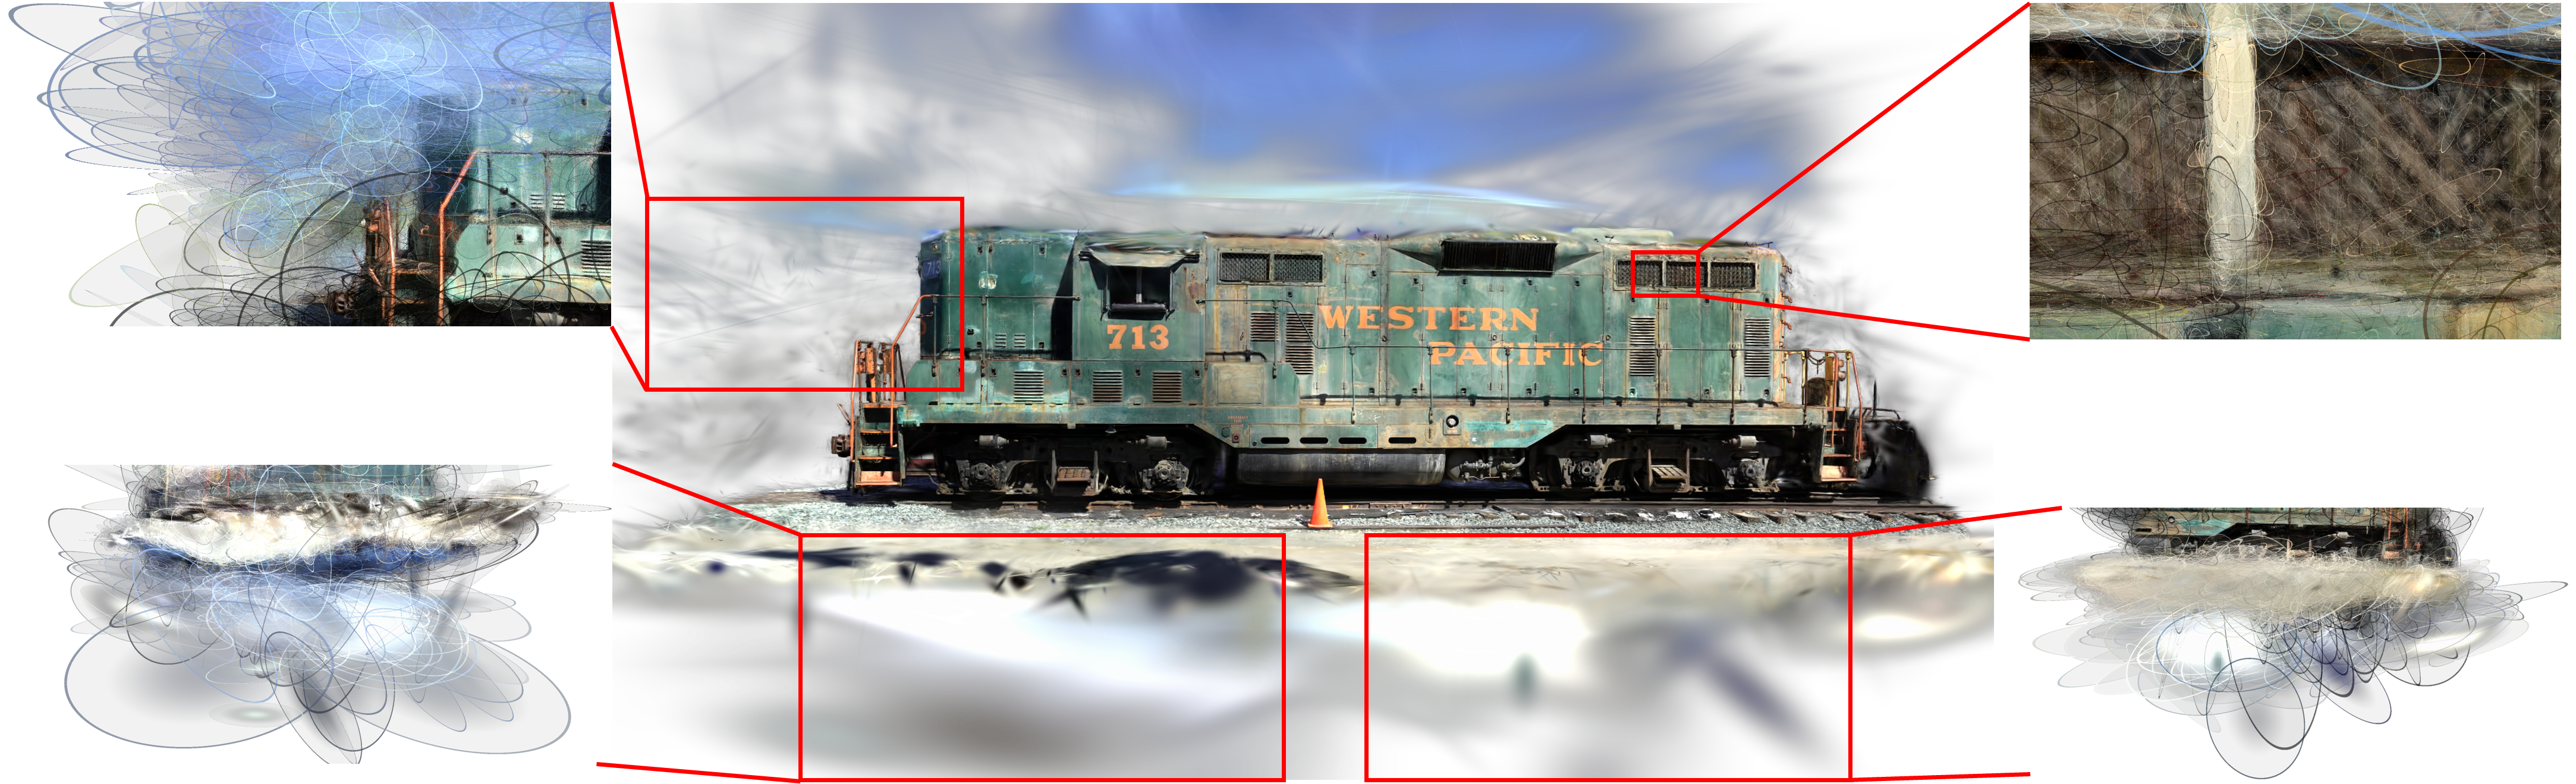
\includegraphics[width=0.8\linewidth]{sec/imgs_main/train_red_vis.png}
  \caption{
  Visualization of redundant and low-importance Gaussians in the \textit{Train} scene from Tanks\&Temples. 
  % Four representative regions are highlighted: 
  % (\textbf{top-left}) numerous floating Gaussians distributed in empty sky regions, indicating spatial isolation; 
  % (\textbf{bottom-left, bottom-right}) clusters of invisible Gaussians generated during densification, where insufficient visibility leads to unoptimized color or SH coefficients; 
  % and (\textbf{top-right}) Gaussians within the same local patch exhibiting large opacity and scale variations. 
  }
  \label{fig:gs_redundancy}
  \vspace{-1.5em}
\end{figure*}

Our key observation, illustrated in Fig.~\ref{fig:gs_redundancy}, is that redundant primitives often exhibit abnormal attributes. For instance, primitives with extremely small scales or very low opacity usually contribute little to rendering quality. Isolated spatial outliers tend to be visually insignificant, though in some cases they may correspond to valid background primitives. Similarly, densification can spawn invisible points with inconsistent colors or near-zero SH coefficients, as they receive little gradient during optimization.
However, no single attribute provides a reliable criterion for importance estimation, as each captures only a limited aspect of information. 
Building on this insight, we propose \textbf{RAP}, a \textbf{R}endering-free \textbf{A}ttribute-guided primitive importance score \textbf{P}rediction framework for estimating primitive importance directly from intrinsic attributes and local neighborhood statistics. Unlike rendering-based or learning-based joint optimization methods, RAP does not require view-dependent computations or per-scene retraining, and also achieves faster calculation with a feedforward style.

Specifically, we extract a 15-dimensional per-point feature vector that captures both global absolute values and local relative statistics, including distance, color, scale, volume, and opacity. 
To model the interactions among these features, we adopt a lightweight MLP that predicts an importance score for each primitive. The network is trained under the supervision of three complementary losses designed to balance fidelity, compactness, and stability: 1) a rendering loss enforces that the pruned model preserves visual fidelity with respect to the ground truth views; 2) A pruning-aware loss prevents the network from trivially assigning high importance to all primitives. This is achieved by regularizing the average predicted score toward a small predefined target, thereby encouraging the network to discard as many primitives as possible and naturally counteracting the rendering loss; 3) A significance distribution regularization ensures that the predicted scores are well separated and distributed from low to high, making downstream tasks, such as pruning decisions, more stable and flexible.
RAP is trained once on a small set of scenes and generalizes well to unseen datasets. Its attribute-based design allows fast, feedforward, plug-and-play importance score prediction without additional scene-specific optimization.  Rendering is only required during the network training, after training, rendering is not necessary for score prediction.

Our contributions are summarized as follows:
\begin{itemize}
    \item We propose RAP, a rendering-free attribute-guided primitive importance score prediction framework that estimates primitive importance directly from intrinsic attributes and local neighborhood statistics.  
    \item We design a set of importance-related per-point features, including average KNN distance, color anisotropy, etc., which together form a compact and discriminative representation of primitive characteristics.  A unified learning framework that based on a lightweight MLP with three tailored loss functions is proposed. These losses jointly constrain the model training, guiding it to produce stable and separable importance score distributions that are friendly to downstream tasks.  
    \item We conduct extensive experiments across diverse datasets and tasks, showing that RAP generalizes well to unseen scenes and consistently improves multiple downstream performance.  
\end{itemize}